\begin{frame}
  \titlepage
\end{frame}

\begin{frame}\frametitle{Motivações na FFLCH}
  Membros da Universidade de São Paulo são também consumidores de sistemas e é comum a multiplicidade de identidade. 
Esse modelo gera problemas para os usuários e para administradores de sistemas na gestão de senhas. \\
Exemplos:
\begin{itemize}
  \item uspdigital
  \item webmail
  \item uspnet
  \item stoa
  \item samba/AD
  \item proxy
  \item \textit{sistema locais}
  \item \textit{sites}
  \item $\infty$
\end{itemize}
\end{frame}

\begin{frame}\frametitle{FFLCH}
Na FFLCH, o Drupal é largamente utilizado nos sites, sendo atualmente 160 instâncias no SaaS Aegir. 
    \begin{figure}
      \caption{\textit{Aegir: deploy and manage many Drupal sites, scale across multiple server clusters. Aegir makes it easy to install, upgrade, and backup an entire network of Drupal sites (Fonte: http://www.aegirproject.org/)} }
      
\includegraphics[width=6cm,height=4cm]{images/aegir-illo.png}
    \end{figure}
\end{frame}

\begin{frame}\frametitle{openLDAP}
Além do Drupal, temos sistemas web internos desenvolvidos pela equipe. 
Usamos por 3 anos o openLDAP para centralização dos usuários. Porém, manter um serviço dessa natureza era muito custozo, dada a rotatividade de pessoas.
(consultas no replicado.)
\begin{figure}
  
\includegraphics[width=4cm,height=2cm]{images/OpenLDAP-logo.png}
\end{figure}
\end{frame}

\begin{frame}\frametitle{OAuth}
\textbf{OAuth} versus \textbf{openLDAP}: O consumer deve conhecer as credenciais do usuário?
\begin{figure}
  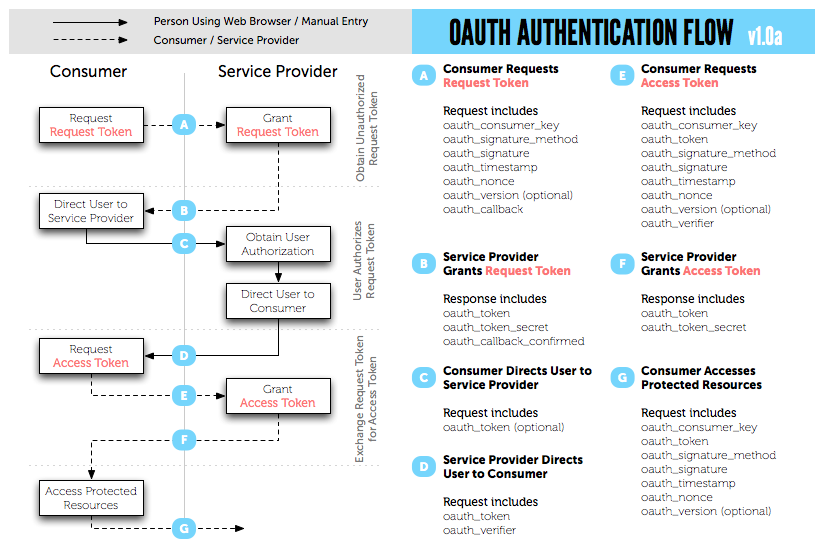
\includegraphics[width=11cm,height=6.5cm]{images/diagram.png}
\end{figure}
\end{frame}

\begin{frame}\frametitle{OAuth na USP e Drupal}
Soubemos da disponibilização do OAuth 1.0 pela lista TI-USP. A implementação em Drupal pode ser feita com módulos contrib do drupal.org: oauth, connector, oauthconnector.  
\begin{block}{Múltiplos sistemas}
Mas como usar o mesmo par consumer key/secret key em diversos sistemas? (dado que confiamos nas aplicações)
\end{block}
\end{frame}


\begin{frame}\frametitle{callback\_id no Drupal}
No cadastro dos consumers é gerado um callback\_id (é mais comum o oauth\_callback). Mas os módulos contribs não previram o envio de outros parâmetros na URL de autorização. \\
O módulo senhaunicausp permite o cadastro e envio de parâmetro callback\_id na URl de autorização.   

git: https://github.com/thigove/senhaunicausp, contribua!
\end{frame}

\begin{frame}[fragile]\frametitle{Implementação do hook\_menu()}
%\lstset{language=PHP}
\begin{lstlisting}
function senhaunicausp_menu(){
  $common = array(
    'file' => 'includes/senhaunicausp.forms.inc'
  );

  $items = array();
    $items['.../callback_id'] = array(
    'title' => t('callback_id'),
    'description' => t('callback_id cadastrado'),
    'page callback' => 'drupal_get_form',
    'page arguments' => array('callback_id_form'),
    'access arguments' => array('senhaunicausp'),
  ) + $common ;

  return $items;	
}
\end{lstlisting}
\end{frame}

\begin{frame}\frametitle{Conclusão}
O OAuth permitiu uma maior integração dos serviços da FFLCH com órgãos centrais da Universidade, 
além de transparecer para o usuário uma maior integração da unidade com a USP. 
\\
Questões em aberto:
\\1) O quão "seguro" é para o usuário usar a mesma identidade em tudo?
\\2) O quão "seguro" é usarmos as mesmas consumer key/secret key em diversos consumers?
\\3) Dados retornado nas APIs do OAuth USP.

\begin{center}
\textbf{Obrigado!!!}
\end{center}

\end{frame}
